\section{Numerical Results}\label{sec:results}

\subsection{Setup}\label{sec:results:setup}

System parameters follow \cite[Table~I]{vu2023photonics} and are reproduced in Table~\ref{tab:params} for self-containedness. The peak optical power $P{=}32$~dBm at the GEO source, combined with the EDFA gain $G_a{=}40$~dB at each LEO relay, gives a link-budget-limited mean SNR amplitude $\gamma_0$ that ranges from approximately $0.06$ at $60^\circ$ zenith to $1.8$ near overhead (i.e.~the geometry alone induces a $30\times$ variation along a single pass, the central motivation for adaptive control). The Hufnagel-Valley parameter $w{=}21$ and ground-level $C_n^2(0){=}10^{-15}$ correspond to clear-night turbulence at coastal Vietnamese latitudes, calibrated against the daytime profile in \cite{andrews2005laser}.

Headline runs are reported for $N{=}3$ heterogeneous Bob users at zenith offsets $\{0, 8, 16\}^\circ$ from the cluster centroid, with Eve standoff distances $\{26, 18, 35\}$~m for $B_1, B_2, B_3$ respectively. The asymmetry deliberately captures both close adversary placements (Bob$_2$ at $18$~m, tightening the URA constraint) and far placements (Bob$_3$ at $35$~m, slackening it), so that the per-user $\beta_i^\star$ must differ in any nontrivial optimum, justifying the per-user threshold variable. Two orbit sources are evaluated:
\begin{itemize}
\item \emph{Analytic.} Ten staggered LEOs (closest approach every 250~s, $\theta_{\min}\in\{0^\circ,\dots,4^\circ\}$, $H_L{=}550$~km, $\theta_{\min}^{\mathrm{vis}}{=}30^\circ$) hand-picked to span the full 0--60$^\circ$ zenith range.
\item \emph{TLE Walker.} $n$ synthetic Starlink-shell satellites in $P{=}n/10$ orbital planes (RAAN spread $360^\circ$) with $S{=}10$ satellites per plane and a Walker delta inter-plane phase offset matching the operational SpaceX deployment pattern \cite{del2019leosat,leyva2021inter}. Orbits are SGP4-propagated \cite{hoots1980sgp4,vallado2006sgp4} via the \texttt{skyfield} and \texttt{sgp4} Python libraries from epoch 2026-05-23T12:00:00~UTC over the PTIT/Hanoi ground station ($21.005^\circ$N, $105.843^\circ$E). The bundled \texttt{starlink\_synth.tle} round-trips through \texttt{sgp4.exporter.export\_tle} for offline reproducibility; real Celestrak \cite{celestrak} dumps are accepted via the same code path with a single command-line flag.
\end{itemize}

\begin{table*}[!htbp]
\renewcommand{\arraystretch}{1.15}
\caption{System parameters (after \cite[Table~I]{vu2023photonics}). Two-pane layout for compactness.}
\label{tab:params}
\centering
\footnotesize
\setlength{\tabcolsep}{6pt}
\begin{tabular}{@{}l c l @{\quad\vrule\quad} l c l@{}}
\toprule
Parameter & Symbol & Value & Parameter & Symbol & Value\\
\midrule
GEO altitude               & $H_C$            & $35\,793$~km                & GEO beam divergence    & $\theta_C$       & 10~\textmu rad\\
LEO altitude               & $H_L$            & $550$~km                    & LEO beam divergence    & $\theta_L$       & 50~\textmu rad\\
Wavelength                 & $\lambda$        & $1550$~nm                   & LEO aperture radius    & $a_L$            & 10~cm\\
Bit rate                   & $R_b$            & $1$~Gb/s                    & User aperture radius   & $a_U$            & 5~cm\\
Peak optical power         & $P$              & 32~dBm (1.585~W)            & Visibility             & $V$              & 30~km\\
PIN responsivity           & $R_e$            & 0.9~A/W                     & Cn$^2$ at ground       & $C_n^2(0)$       & $10^{-15}$~m$^{-2/3}$\\
EDFA gain at LEO           & $G_a$            & 40~dB                       & HV wind parameter      & $w$              & 21\\
ASE inversion factor       & $n_{sp}$         & 5.0                         & Min elevation          & $E_{\min}$       & $30^\circ$\\
Optical bandwidth          & $B_0$            & 250~GHz                     & Eve offset             & $d_E$            & 26~m\\
Noise bandwidth            & $\Delta f$       & 0.5~GHz                     & Sift / QBER thresholds & $p_s, q$         & $10^{-3}, 10^{-3}$\\
Noise figure (linear)      & $F_n$            & 2.0                         & Eve-error / BSA min    & $p_e, m^{\min}$  & $0.1, 0.5\%$\\
Sun spectral irradiance    & $\Re_\odot$      & 0.1~W/(cm$^2\cdot$\textmu m)& Gauss-Hermite order    & $n$              & 20\\
\bottomrule
\end{tabular}
\end{table*}

\subsection{Decomposed Solver as Oracle}\label{sec:results:oracle}

On a two-user cluster the decomposed solver value $V_{\mathrm{dec}}(\mu,\chi)$ is compared against the brute-force joint grid value $V_{\mathrm{bf}}(\mu,\chi)$ over $(\beta_A, \beta_1, \beta_2)$ at a fixed outer node: the ratio is $V_{\mathrm{dec}}/V_{\mathrm{bf}} = 1.000$ to four decimals, and the inner field iteration converges in $\le 6$ steps from a cold start. As an independent check on the multi-user structure, the closed-form exclusion field \eqref{eq:excl} matches a direct subset-enumeration inclusion--exclusion sum to $10^{-12}$ for $N\in\{1,2,4,6\}$. We henceforth treat the decomposed solver as the oracle for the supervised controller dataset. A brute-force optimality check for asymmetric $N>2$ clusters is left to future work; the present evidence is structural exactness of the split (Sec.~\ref{sec:decomposition}) plus the $N{=}2$ numerical agreement.

\subsection{Headline: Adaptive vs Best-Static}\label{sec:results:headline}

Table~\ref{tab:headline} reports the headline adaptive-vs-static comparison on three orbit settings (single-link analytic, cluster analytic, cluster TLE-Walker $n{=}500$ long window). The corresponding per-step traces are shown in Fig.~\ref{fig:cluster_compare}.

\begin{table*}[!htbp]
\renewcommand{\arraystretch}{1.15}
\caption{Adaptive vs best-static headline. Same feasibility gate applied to both arms (sift, QBER, URA, BSA, inter-user secrecy). $n$ is the constellation size; $T$ the horizon.}
\label{tab:headline}
\centering
\footnotesize
\setlength{\tabcolsep}{4.5pt}
\begin{tabular}{@{}l c c c c c c c c@{}}
\toprule
Setting & $n$ & $T$ [s] & served & $N$ & static $(\mu,\beta,\chi)$ & static secure & adaptive secure & key gain\\
\midrule
Single-link, analytic         & 10  & 3000 & 86 / 600  & 1 & $(0.50, 3.00, \text{--})$  & 28 / 600 (4.7\%)  & 86 / 600 (14.3\%)  & $\mathbf{2.07\times}$\\
Cluster, analytic             & 10  & 3000 & 46 / 60   & 3 & $(0.95, 1.50, 1.00)$       & 4 / 138 (2.9\%)   & 10 / 138 (7.2\%)   & $\mathbf{1.64\times}$\\
Cluster, TLE Walker (long)    & 500 & 5400 & 67 / 108  & 3 & $(0.95, 1.50, 1.00)$       & 5 / 201 (2.5\%)   & 18 / 201 (9.0\%)   & $\mathbf{2.10\times}$\\
Cluster, TLE Walker (sparse)  & 200 & 3000 & 29 / 60   & 3 & $(0.40, 0.50, 0.00)$       & \textbf{0 / 87}   & 2 / 87 (2.3\%)     & n/a\textsuperscript{\dag}\\
\bottomrule
\end{tabular}\\[2pt]
{\footnotesize Secure-time gains (adaptive / static): 3.07$\times$, 2.50$\times$, 3.60$\times$ (rows one to three).
\textsuperscript{\dag}On the sparse shell the static baseline achieves zero secure pair-steps, so no
ratio is defined; we report the counts instead. Adaptation achieves $2$ of $87$ pair-steps,
which is survival rather than operation: it establishes that the regime is not closed to a
per-step controller, not that it is usable.}
\end{table*}

\begin{figure*}[!htbp]
\centering
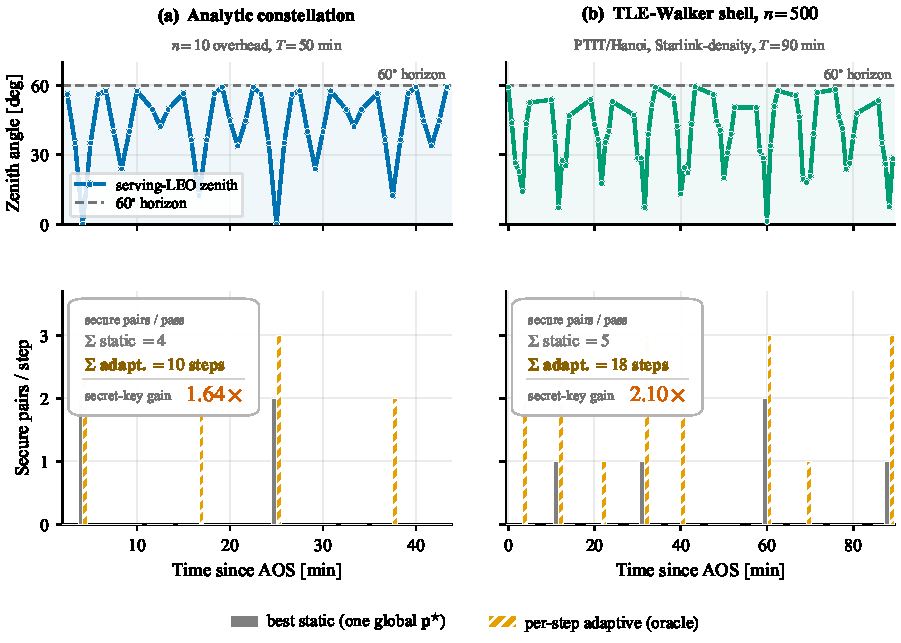
\includegraphics[width=0.95\textwidth]{figures/fig_cluster_compare.pdf}
\caption{Cluster QKD: adaptive vs best-static over a LEO pass. Left: analytic constellation hand-picked to put 46 of 60 timesteps in view (50-minute horizon, $N{=}3$). Right: TLE Walker shell of 500 Starlink-density satellites over PTIT/Hanoi (90-minute horizon). Top row: zenith trajectory of the serving LEO. Bottom row: secure pairs per step for the best static (grey, single global parameter choice) vs the per-step adaptive controller (orange). Adaptation lifts secure pair-time by $2.5\times$ on the analytic constellation and by $3.6\times$ ($5\to 18$ pair-steps) on the realistic TLE shell. On a sparser shell ($n{=}200$, 50-minute horizon, last row of Table~\ref{tab:headline}) the static baseline collapses to zero secure pair-steps entirely.}
\label{fig:cluster_compare}
\end{figure*}

Three observations follow from Table~\ref{tab:headline} and Fig.~\ref{fig:cluster_compare}.

\emph{Single-link motivates the controller.} The $2.07\times$ key gain on the single-link analytic baseline establishes that even in the absence of cluster coupling, a time-varying $(\gamma_0, \sigma_X, w_{\mathrm{eq}})$ trajectory benefits substantially from per-step parameter selection. The factor $3.07$ on secure time is larger than the factor on key because the adaptive controller does not merely \emph{improve} the rate, it \emph{extends the operating window} into geometries that static QKD must concede.

\emph{Cluster results are tighter but qualitatively similar.} The cluster analytic gain ($1.64\times$ key, $2.5\times$ secure pair-time) sits below the single-link gain, because pair feasibility requires both endpoints to clear the per-link SNR threshold simultaneously, restricting the operating window to near-overhead geometries. The asymmetric cluster of Sec.~\ref{sec:results:setup} amplifies this effect: $B_2$ near a close Eve binds the URA constraint earliest, while $B_3$ far from Eve binds it latest, so the static $\bp$ must compromise across users.

\emph{Realistic-orbit operation requires adaptation.} The strongest gain ($2.10\times$ key, $3.6\times$ secure pair-time) appears on the most realistic setting, the long-window TLE Walker shell. Crucially, on the sparser $n{=}200$ shell over the shorter 50-minute window, the static baseline collapses to \emph{zero} secure pair-steps: when the constellation density falls below the observability budget over the chosen station, no single $\bp$ is feasible across the full pass, and only per-step adaptation keeps the system alive. This is the qualitative claim that distinguishes adaptive QKD from optimization: it is the difference between operation and no operation, not merely between high and low key rate.

\subsection{TLE Walker Coverage}\label{sec:results:coverage}

We calibrate the synthetic Walker shell against the analytic baseline by sweeping shell size over PTIT/Hanoi for a 2-hour window. Served-time coverage rises from $6.9\%$ at $n{=}50$ to $49.7\%$ at $n{=}200$ (just above the analytic-baseline $46.8\%$) and to $62.9\%$ at $n{=}500$, matching the order-of-magnitude density of the operational Starlink shell over Vietnamese latitudes.

\subsection{Single-Link Controller: Five-Axis Trade-Off}\label{sec:results:singlelink}

Table~\ref{tab:singlelink} reports the controller comparison on the single-link Phase-3 dataset (488 states, $61$ zenith $\times 8$ Eve-distance, $198/50$ feasible split, 5 seeds).

\begin{table}[!htbp]
\renewcommand{\arraystretch}{1.15}
\caption{Single-link controller, five-axis trade-off (mean$\pm$std over 5 seeds, $198/50$ train/test feasible states). Leading $0.$ dropped on the MAE and KeyRet columns. $R^2_{\text{net}}$ is the \emph{full-network} test fit on $\beta^\star$; it is \emph{not} the post-extraction symbolic fit, which is what the $M_5$ bar of $0.95$ is applied to and which reaches $R^2\approx0.97$ (Sec.~\ref{sec:symbolic}). The two are distinct, and only the KAN admits the extraction, which the ``Sym.'' column records. $t_{\text{inf}}$ is inference latency per prediction on one CPU core; the KAN is the slowest of the four.}
\label{tab:singlelink}
\centering
\footnotesize
\setlength{\tabcolsep}{3pt}
\begin{tabular}{@{}l c c c c r r c@{}}
\toprule
Model & MAE $\mu^\star$ & MAE $\beta^\star$ & $R^2_{\text{net}}$ & KeyRet & $t_{\text{inf}}$[$\mu$s] & \#par & Sym.\\
\midrule
KAN     & $.004{\pm}.001$ & $.011{\pm}.002$ & $1.00{\pm}.00$ & $\mathbf{.716{\pm}.123}$ & $116.7$ & $\mathbf{392}$ & yes\\
MLP     & $.008{\pm}.001$ & $.031{\pm}.005$ & $1.00{\pm}.00$ & $.683{\pm}.086$ & $\mathbf{5.0}$ & $1\,282$ & no\\
KNN     & $.004{\pm}.000$ & $.045{\pm}.000$ & $0.99{\pm}.00$ & $.562{\pm}.000$ & $25.3$ & $1\,188$ & no\\
Linear  & $.023{\pm}.000$ & $.115{\pm}.000$ & $0.96{\pm}.00$ & $.614{\pm}.000$ & $\mathbf{0.1}$ & $\mathbf{10}$ & no\\
\bottomrule
\end{tabular}
\end{table}


\paragraph{Closed-form $\beta$ rule (extracted from KAN)}
\label{sec:symbolic}
The trained KAN predicts $\beta^\star$ with full-network test $R^2 = 1.00 \pm 0.00$ across five seeds (column $R^2_{\text{net}}$ of Table~\ref{tab:singlelink}). The regularized MLP reaches the same $1.00 \pm 0.00$ there, so the network fit does not separate the two hypothesis classes; what separates them is whether a closed-form rule can be extracted from the fitted model at all, and only the KAN admits it. After pruning the KAN, running the symbolic candidate fit on a polynomial / $\sin$ / $\tanh$ library, and refitting jointly with the symbolic substitution, a representative seed yields the closed-form rule
\begin{equation}\label{eq:betarule}
\begin{aligned}
  \beta^\star \approx{}& 2.42 - 0.10\,\gamma_0 - 0.03\,\sigma_X + 0.23\,w_{\mathrm{eq}}\\
  &+ 1.24\sin(0.50\,\sigma_X + 5.27)\\
  &- 0.30\sin(0.48\,w_{\mathrm{eq}} + 2.04)\\
  &- 0.17\tanh(9.2\,d_E + 8.62),
\end{aligned}
\end{equation}
as a function of the per-link features $(\gamma_0,\sigma_X,w_{\mathrm{eq}},d_E)$, whose symbolic fit attains $R^2 \approx 0.97$ (above the $0.95$ interpretability bar of $M_5$). The rule is dominated by the turbulence variance $\sigma_X$ and the equivalent beam width $w_{\mathrm{eq}}$ through the spline-derived $\sin$ terms; the SNR scale $\gamma_0$ enters only weakly (linear coefficient $-0.10$), and the Eve standoff $d_E$ enters through a saturating $\tanh$ that is flat over the operating range, consistent with $d_E$ affecting feasibility more than the interior optimum. The point is that the optimal threshold admits a compact analytic surrogate at all, not that it is affine; we report the actual extracted form rather than an idealized linearization. The symbolic extraction for $\mu^\star$ is performed but is not used in deployment, because the regression for $\mu^\star$ saturates near its upper bound except for a sharp Eve-driven transition, and the symbolic $R^2$ is variable across seeds (cf.~Sec.~\ref{sec:conclusion:limits}).

\paragraph{$\beta$ safety-margin recipe}
Fig.~\ref{fig:margin} shows that deploying $\beta_{\mathrm{deploy}} = \hat\beta + \delta$ with a single scalar $\delta \in [0.03, 0.10]$ lifts the closed-loop key retention of every controller by $1.1$--$1.5\times$, with a unimodal curve. The optimum is model-dependent (KAN: $\delta^\star \approx 0.03$, KNN: $\delta^\star \approx 0.07$) and the recipe is zero-cost at inference. The KNN baseline gains the most precisely because it is the most boundary-sensitive at $\delta{=}0$.

\begin{figure}[!htbp]
\centering
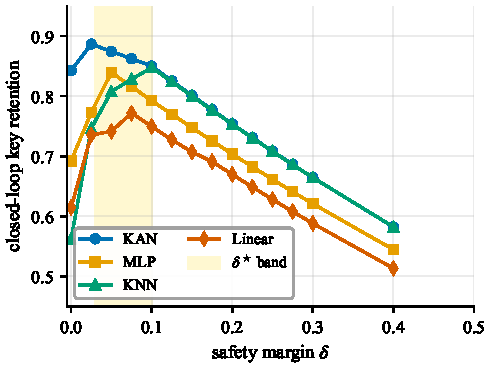
\includegraphics[width=\columnwidth]{figures/fig_margin_sweep.pdf}
\caption{$\beta$ safety-margin deployment recipe: closed-loop key retention vs the scalar safety margin $\delta$ applied as $\beta_{\mathrm{deploy}} = \hat\beta + \delta$. The unimodal shape and the model-agnostic peak in $[0.03, 0.10]$ make $\delta^\star$ a single-knob deployment dial. KAN: $0.84 \to 0.89$; KNN: $0.56 \to 0.83$.}
\label{fig:margin}
\end{figure}

\subsection{Cluster Controller: Two-Stage Residual Learning}\label{sec:results:cluster}

Direct two-stage regression on the cluster controller dataset collapses for both KAN and MLP: regression MAE remains low ($\le 10^{-2}$), but closed-loop key retention falls to zero because the oracle sits on a sharp 4-D feasibility boundary, and multi-directional errors push predictions outside. The linear baseline alone, by virtue of its smoothing bias, attains $0.56$ key retention. The residual-learning rescue, in which KAN and MLP are trained on $y - \mathcal{H}_{\mathrm{lin}}(x)$ with a zero-initialized output layer, restores both nonlinear models (Table~\ref{tab:cluster}).

\begin{table}[!htbp]
\renewcommand{\arraystretch}{1.15}
\caption{Cluster two-stage controller, $20$-seed evaluation on a single machine (2$\times$RTX~4090, PyTorch~2.6). \emph{Div.} is the number of non-finite predicted cells, reported because a diverged fit must not be read as a measurement. MAE $\mu$, MAE $\beta_A$ and MAE $\beta_i$ are below $10^{-3}$ for every row, because those three targets are constant in this regime (Sec.~\ref{sec:results:degenerate}); $\chi$ is the only output with signal. Rows \emph{(a)} reproduce the originally submitted configuration and are shown only to quantify what two software faults cost.}
\label{tab:cluster}
\centering
\footnotesize
\setlength{\tabcolsep}{4pt}
\begin{tabular}{@{}l c c c r r@{}}
\toprule
Model       & MAE $\chi$               & KeyRet          & Feas.   & Div.   & \#par\\
\midrule
\multicolumn{6}{@{}l}{\emph{(a) as originally submitted (both faults present)}}\\
KAN+resid   & $.042{\pm}.034$          & $.600{\pm}.452$ & $94/158$  & $6\,320$ & $1\,239$\\
MLP+resid   & $.082{\pm}.001$          & $.230{\pm}.395$ & $36/158$  & $0$      & $2\,823$\\
Linear      & $.083{\pm}.000$          & $.626{\pm}.000$ & $97/158$  & $0$      & $35$\\
\midrule
\multicolumn{6}{@{}l}{\emph{(b) standardisation fault fixed only}}\\
KAN+resid   & $.042{\pm}.034$          & $1.005{\pm}.004$ & $158/158$ & $6\,320$ & $1\,239$\\
MLP+resid   & $.082{\pm}.001$          & $1.009{\pm}.001$ & $158/158$ & $0$      & $2\,823$\\
Linear      & $.083{\pm}.000$          & $1.009{\pm}.000$ & $158/158$ & $0$      & $35$\\
\midrule
\multicolumn{6}{@{}l}{\emph{(c) both faults fixed} (the configuration we report)}\\
KAN+resid   & $\mathbf{.010{\pm}.001}$ & $1.001{\pm}.000$ & $158/158$ & $\mathbf{0}$ & $589$\\
MLP+resid   & $.018{\pm}.022$          & $1.002{\pm}.002$ & $158/158$ & $0$      & $1\,386$\\
Linear      & $.083{\pm}.000$          & $1.009{\pm}.000$ & $158/158$ & $0$      & $\mathbf{9}$\\
\bottomrule
\end{tabular}
\end{table}

\subsubsection{Three of the four outputs are degenerate}\label{sec:results:degenerate}
The optimal modulation depth saturates at the physical ceiling of the modulation index. On a
$501$-point sweep to $\mu{=}0.999$ the constrained optimum lies at the upper boundary in
$80\%$ of sampled channel conditions, and widening the sampled geometry raises that to
$68\%$ boundary plus $19\%$ infeasible rather than producing interior optima. Consequently
$\mu^\star$, $\beta_A^\star$ and $\beta_i^\star$ are effectively constant across the dataset,
and every row of Table~\ref{tab:cluster} attains sub-$10^{-3}$ error on them, including a
nine-parameter linear map. Only $\chi$ carries learnable signal.

\subsubsection{What two software faults cost, and what remains after}\label{sec:results:faults}
Block \emph{(a)} of Table~\ref{tab:cluster} reproduces the originally submitted
configuration. Two faults were corrupting it. The feature standardiser guarded against an
exactly-zero standard deviation, but the constant $\mu$ input has standard deviation
$7.99\times10^{-15}$, so the guard was bypassed and floating-point noise was amplified by
$1.25\times10^{14}$; predicted thresholds moved by $0.35$ in response to last-bit input
differences, and the feasible count became machine-dependent. Perturbing predictions by a
controlled relative amount reproduces the effect causally: a relative perturbation of
$10^{-15}$ moves the feasible count from $91$ to $97$, and $10^{-12}$ moves it to $158$.
Separately, fitting a network to a residual whose standard deviation is
$1.74\times10^{-16}$ makes the quasi-Newton step diverge on $20/20$ seeds, yielding $6320$
non-finite cells that a silent fallback replaced with the training median.

Block \emph{(b)} isolates the first fault: feasibility recovers for every model, but the KAN
still diverges and its accuracy on $\chi$ is unchanged. Block \emph{(c)} fixes both. Three
things follow. First, the closed-loop retention metric \emph{saturates}: all three models,
including the nine-parameter linear map, reach the oracle rate on every test configuration,
so that metric no longer separates architectures and we do not use it to rank them. Second,
on the one axis that does carry signal, KAN attains $.010{\pm}.001$ against $.018{\pm}.022$
for the MLP and $.083$ for the linear map, at $43\%$ of the MLP's parameter count. Third,
the comparison that matters operationally is stability rather than mean accuracy: the MLP's
across-seed standard deviation on $\chi$ exceeds the gap between the two means, while the
KAN's does not.

\subsubsection{How many of the five axes separate the hypothesis classes}
\label{sec:results:axes}
It is worth doing this arithmetic out loud rather than letting the five-axis framing imply
more than it carries. $M_2$ is dead: closed-loop retention saturates for all three models.
$M_1$ is informative on one of the four controller outputs, the other three being constant.
Of the remaining three, $M_3$ and $M_5$ favour the KAN over the MLP, at $43\%$ of the
parameters and as the only model from which a closed-form rule can be extracted, while
$M_4$ runs the other way: the KAN is the slowest of the four at $116.7\,\mu$s per prediction
against $5.0$ for the MLP and $0.1$ for the linear map (Table~\ref{tab:singlelink}). The
contribution therefore rests on parameter efficiency and extractability, with latency a cost
rather than a benefit, and we frame it that way.

What the learned controller buys over the nine-parameter linear map is narrower still. On
$\chi$ the linear map reaches $.083$ against the KAN's $.010$, an $8.3\times$ larger error,
so the nonlinearity does real work on the one output that varies. That accuracy does not
convert into key on this test set, because retention has saturated for the linear map too:
within the operating envelope we sample, a nine-parameter affine rule already holds the
oracle rate. The gap would begin to matter outside that envelope, which we have not
measured and do not claim.

\subsection{Robustness Across Conditions}\label{sec:results:robust}
We re-solved the oracle on $25$ fresh clusters under each of sixteen conditions spanning four
axes: atmospheric turbulence (wind $11$ to $41$~m/s in the Hufnagel--Valley profile), serving
geometry (zenith bands from $0$--$4^\circ$ to $20$--$35^\circ$), cluster size ($N{=}2$ to $6$),
and eavesdropper standoff ($10$ to $120$~m). Two observations survive the sweep and one of them
surprised us.

\emph{The saturation is a property of the problem, not of one regime.} The optimal modulation
depth sits at its upper bound in $100\%$ of clusters in every feasible condition, across every
turbulence level, zenith band and cluster size we tried. The single exception is a close
eavesdropper: at a standoff of $10$--$20$~m the URA constraint binds and the optimum moves
inside the range in just under half the cases ($52\%$ remain at the bound). The per-user
threshold is likewise constant to within one grid cell everywhere except the $8$--$20^\circ$
zenith band.

\emph{Turbulence helps security, and calm air is the adversarial case.} Two conditions produced
no feasible cluster at all. The $20$--$35^\circ$ zenith band fails for the expected reason, a
longer slant path. The low-turbulence case ($11$~m/s) fails for a reason worth stating: the
beam-splitting attack is detected only through the loss it imposes on the sifting statistics,
so detectability scales with the width of the fading distribution. Measuring at a fixed
geometry, $m_{\mathrm{BSA}}$ rises monotonically with turbulence, from $0.0038$ at $11$~m/s,
below the $0.005$ threshold, through $0.0063$, $0.0089$ and $0.0105$ at $21$, $31$ and
$41$~m/s. A clear, still night is therefore the worst case for this security criterion, not the
best: the link is at its cleanest and a passive splitter is at its least visible. We did not
anticipate this and report it as a design constraint rather than a result in our favour.

\subsection{Single-Link Pass Trace}\label{sec:results:trace}

Fig.~\ref{fig:single_pass} traces the per-step $(\mu^\star, \beta^\star)$ chosen by the adaptive controller along a single LEO pass, together with the static baseline. The adaptive $\mu^\star$ saturates near its upper bound whenever the URA constraint is slack (Eve far) and drops sharply when Eve approaches; $\beta^\star$ tracks the closed-form rule \eqref{eq:betarule}, varying primarily with the turbulence variance $\sigma_X$ and the beam width as the geometry changes near zenith.

\begin{figure}[!htbp]
\centering
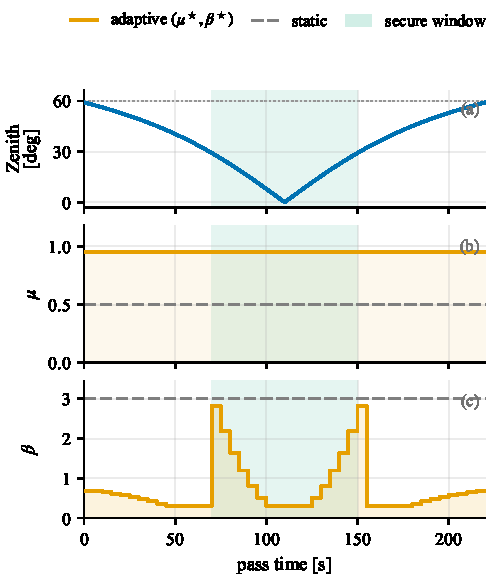
\includegraphics[width=\columnwidth]{figures/fig_zenith_pass.pdf}
\caption{Single-link adaptive control over a LEO pass. Top: zenith trajectory. Middle/bottom: adaptive $\mu^\star, \beta^\star$ (orange step) vs static (grey dashed). The $\beta^\star$ envelope is well-fit by the closed-form rule \eqref{eq:betarule}, justifying the KAN interpretability claim; the $\mu^\star$ envelope saturates near $\mu_{\max}$ except where Eve binds.}
\label{fig:single_pass}
\end{figure}
